%
% carlson.tex
%
% (c) 2022 Prof Dr Andreas Müller, OST Ostschweizer Fachhochschule
%
\subsection{Der Satz von Carlson
\label{buch:funktionentheorie:subsection:satz-von-carlson}}
In Abschnitt~\ref{buch:rekursion:section:gamma} wurde gezeigt,
wie die Gamma-Funktion $\Gamma(x)$ konstruiert werden kann, die
in ganzzahligen Argumenten mit der Fakultät zusammenfällt.
Es wurde auch gezeigt, dass $\Gamma(x)+\sin(\pi x)$ eine
weitere Funktion mit dieser Eigenschaft ist.
Die Integraldefinition der
Gamma-Funktion~\ref{buch:rekursion:def:gamma} zeigt, dass
die Gamma-Funktion holomorph ist.
Der folgende Satz von Carlson zeigt jetzt, dass sich
zwei solche Lösungen um eine unbeschränkte Funktion
unterscheiden müssen.

\begin{satz}[Carlson]
\label{buch:funktionentheorie:satz:carlson}
Ist $f(z)$ eine holomorphe Funktion, die für $\operatorname{R}z\ge 0$
beschränkt ist und an den Stellen $z=1,2,3,\dots$ verschwindet.
Dann ist $f(z)=0$.
\end{satz}

\index{Satz!von Carlson}%
\index{Carlson, Satz von}%
\begin{figure}
\centering
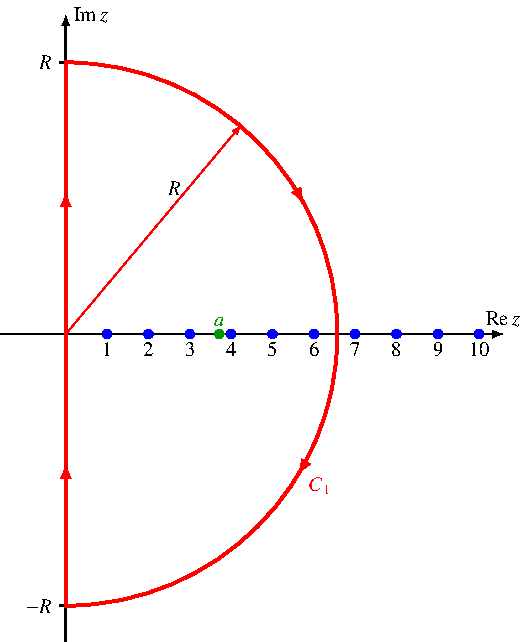
\includegraphics{chapters/080-funktionentheorie/images/carlsonpath.pdf}
\caption{Pfad zum Beweis des Satzes \ref{buch:funktionentheorie:satz:carlson}
von Carlson.
\label{buch:funktionentheorie:fig:carlsonpath}}
\end{figure}

\begin{proof}[Beweis]
Da $f(1)=f(2)=f(3)=\dots=0$ ist auch die Funktion
\[
g_n(z) = \frac{f(z)}{(z-1)(z-2)\cdot\ldots\cdot(z-n)}
\]
eine holomorphe Funktion.
Für $|z|>n$ ist jeder Faktor im Nenner betragsmässig $>1$,
also ist $g_n(z)$ in der rechten Halbebene nicht nur beschränkt,
es gilt sogar
\[
|g_n(z)| =\frac{|f(z)|}{|z-1|\cdot|z-2|\cdot\ldots\cdot|z-n|}
\le \frac{M}{(|z|-n)^n}
=
O\biggl(\frac{1}{|z|^n}\biggr)
\qquad\text{für $|z|\to\infty$}.
\]
Mit dem Cauchy-Integralsatz kann man jetzt $g_n(a)$ für einen
Punkt $a$ in der rechten Halbebene berechnen, er ist
\begin{equation}
g_n(a)
=
\frac{1}{2\pi i}
\oint_{\gamma} \frac{g_n(z)}{z-a}\,dz
=
\frac{f(a)}{(a-1)(a-2)\cdot\ldots\cdot(a-n)},
\label{buch:funktionentheorie:proof:eqn:gna}
\end{equation}
wobei $\gamma$ ein Pfad ist, der $a$ umschliessen muss.

Als Pfad wählen wir einen Halbkreis $C_1$ vom Radius $R$ um den Nullpunkt
und das Segment von $-iR$ bis $iR$, dargestellt in
Abbildung~\ref{buch:funktionentheorie:fig:carlsonpath}.
% XXX Bild des Pfades
Das Integral über den Halbkreis kann durch
\begin{align*}
\biggl|
\frac{1}{2\pi i}
\int_{C_1} \frac{f(z)}{(z-a)(z-1)(z-2)\cdot\ldots\cdot(z-n)}\,dz
\biggr|
&\le
\frac1{2\pi} \max_{|z|=R\wedge\operatorname{Re}z\ge 0}
\frac{M}{|z-a|\cdot|z-1|\cdot|z-2|\cdot\ldots\cdot|z-n|}\pi R
\\
&\le
\frac{M\pi R}{(R-n)^n}
\end{align*}
abgeschätzt werden.
Die rechte Seite geht für $n>1$ gegen $0$ wenn $R\to\infty$ geht.
Das Integral über den Kreisbogen $C_1$ trägt also nichts bei zum
Integral~\eqref{buch:funktionentheorie:proof:eqn:gna}

Es bleibt das Integral über die imaginäre Achse, es ist
\begin{align}
g_n(a)
&=
\frac{1}{2\pi i}
\int_{-\infty}^\infty
\frac{f(it)}{(it-a)(it-1)(it-2)\cdot\ldots\cdot(it-n)}
\,i\,dt
\notag
\\
|g_n(a)|
&=
\frac{1}{2\pi}
\int_{-\infty}^\infty
\frac{|f(it)|}{
\sqrt{(a^2+t^2)(1^2+t^2)(2^2+t^2)\cdot\ldots\cdot(n^2+t^2)}
}
\,dt.
\notag
\intertext{Im Nenner kann man in den Faktoren $(k^2+t^2)$ mit $k>1$
das $k^2$ weglassen, was den Nenner kleiner und damit den ganzen Ausdruck
grösser macht.
Es bleibt dann nur noch der erste Term, in dem wir $a>1$ durch $1$ ersetzen
können.
Insgesamt bekommen wir so die Abschätzung}
&\le
\frac{1}{2\pi} \int_{-\infty}^\infty
\frac{M}{\sqrt{(1+t^2)(1+t^2)}\cdot 2\cdot 3\cdot\ldots\cdot n}
\,dt
=
\frac{M}{2\pi n!}
\int_{-\infty}^\infty\frac{dt}{1+t^2}
=
\frac{M}{2 n!}.
\label{buch:funktionentheorie:carlson:eqn:integral}
\end{align}
Um eine Abschätzung für $f(a)$ zu erhalten, muss man jetzt noch den Nenner
von \eqref{buch:funktionentheorie:proof:eqn:gna} abschätzen.
Da $a$ nicht ganzzahlig ist, ist die nächstkleiner Ganzzahl $[a]\ne a$.
Das Produkt im Nenner von \eqref{buch:funktionentheorie:proof:eqn:gna}
kann daher aufgespaltet werden in die Faktoren $(a-k)$ mit $k<a$ und
die Faktoren  mit $k>a$.
Den Betrag der Faktoren mit $k<a$ kann man vergrössern, indem man $a$
durch $[a]+1$ ersetzt, man erhält
\begin{align*}
|
(a-1)(a-2)\cdots(a-[a])
|
&\le
([a]+1-1)([a]+1-2)\cdots([a]+1-[a])=[a]!.
\intertext{Die nachfolgenden Faktoren kann man vergrössern, indem man $a$ durch $[a]$ ersetzt, was}
|(a-([a]+1))(a-([a]+2))\cdots(a-n)|
&\le
|([a]-([a]+1))([a]-([a]+2))\cdots([a]-n)|
\\
&=
1\cdot 2 \cdot\ldots\cdot |n-[a]|
=
(n-[a])!.
\end{align*}
ergibt.
Aus \eqref{buch:funktionentheorie:proof:eqn:gna} und der Abschätzung
\eqref{buch:funktionentheorie:carlson:eqn:integral}
für $|g_n(a)$
erhält man jetzt
\[
|f(a)|
=
|(a-1)(a-2)\cdots(a-n)|\cdot|g_n(a)|
\le 
\frac{[a]!\,(n-[a])!}{n!}
\frac{M}{2}
=
\frac{M}{2} \binom{n}{[a]}^{-1}.
\]
Für $n>[a]$ ist der Binomialkoeffizient auch $>n$ und somit
\[
|f(a)|\le \frac{M}{2n}
\to 0
\qquad\text{für $n\to\infty$}.
\]
Damit ist gezeigt, dass $f(a)=0$ ist für alle reellen $a>1$.
A fortiori verschwinden auch alle Ableitungen von $f$ und damit
damit auch die zugehörige Potenzreihe, also $f(z)=0$.
\end{proof}

